\documentclass[11pt]{article}
\renewcommand{\arraystretch}{1.5} % Default value: 1
\usepackage{sectsty}
\allsectionsfont{\color{blue}\fontfamily{lmss}\selectfont}
\usepackage{fontspec}
\setmainfont{XCharter}

\usepackage{listings}
\lstset{
basicstyle=\small\ttfamily,
tabsize=8,
columns=flexible,
breaklines=true,
frame=tb,
rulecolor=\color[rgb]{0.8,0.8,0.7},
backgroundcolor=\color[rgb]{1,1,0.91},
postbreak=\raisebox{0ex}[0ex][0ex]{\ensuremath{\color{red}\hookrightarrow\space}}
}
\usepackage{fontawesome}


\usepackage{mdframed}
\newmdenv[
  backgroundcolor=gray,
  fontcolor=white,
  nobreak=true,
]{terminalinput}



\usepackage{parskip}




    \usepackage[T1]{fontenc}
    % Nicer default font (+ math font) than Computer Modern for most use cases
    \usepackage{mathpazo}

    % Basic figure setup, for now with no caption control since it's done
    % automatically by Pandoc (which extracts ![](path) syntax from Markdown).
    \usepackage{graphicx}
    % We will generate all images so they have a width \maxwidth. This means
    % that they will get their normal width if they fit onto the page, but
    % are scaled down if they would overflow the margins.
    \makeatletter
    \def\maxwidth{\ifdim\Gin@nat@width>\linewidth\linewidth
    \else\Gin@nat@width\fi}
    \makeatother
    \let\Oldincludegraphics\includegraphics
    % Set max figure width to be 80% of text width, for now hardcoded.
\renewcommand{\includegraphics}[1]{\Oldincludegraphics[width=.8\maxwidth, height=.55\textheight, keepaspectratio]{#1}}
    % Ensure that by default, figures have no caption (until we provide a
    % proper Figure object with a Caption API and a way to capture that
    % in the conversion process - todo).
    \usepackage{caption}
    \DeclareCaptionLabelFormat{nolabel}{}
    \captionsetup{labelformat=nolabel, textfont=bf}

    \usepackage{adjustbox} % Used to constrain images to a maximum size
    \usepackage{xcolor} % Allow colors to be defined
    \usepackage{enumerate} % Needed for markdown enumerations to work
    \usepackage{geometry} % Used to adjust the document margins
    \usepackage{amsmath} % Equations
    \usepackage{amssymb} % Equations
    \usepackage{textcomp} % defines textquotesingle
    % Hack from http://tex.stackexchange.com/a/47451/13684:
    \AtBeginDocument{%
        \def\PYZsq{\textquotesingle}% Upright quotes in Pygmentized code
    }
    \usepackage{upquote} % Upright quotes for verbatim code
    \usepackage{eurosym} % defines \euro
    \usepackage[mathletters]{ucs} % Extended unicode (utf-8) support
    \usepackage[utf8x]{inputenc} % Allow utf-8 characters in the tex document
    \usepackage{fancyvrb} % verbatim replacement that allows latex
    \usepackage{grffile} % extends the file name processing of package graphics
                         % to support a larger range
    % The hyperref package gives us a pdf with properly built
    % internal navigation ('pdf bookmarks' for the table of contents,
    % internal cross-reference links, web links for URLs, etc.)
    \usepackage{hyperref}
    \usepackage{longtable} % longtable support required by pandoc >1.10
    \usepackage{booktabs}  % table support for pandoc > 1.12.2
    \usepackage[inline]{enumitem} % IRkernel/repr support (it uses the enumerate* environment)
    \usepackage[normalem]{ulem} % ulem is needed to support strikethroughs (\sout)
                                % normalem makes italics be italics, not underlines




    % Colors for the hyperref package
    \definecolor{urlcolor}{rgb}{0,.145,.698}
    \definecolor{linkcolor}{rgb}{.71,0.21,0.01}
    \definecolor{citecolor}{rgb}{.12,.54,.11}

    % ANSI colors
    \definecolor{ansi-black}{HTML}{3E424D}
    \definecolor{ansi-black-intense}{HTML}{282C36}
    \definecolor{ansi-red}{HTML}{E75C58}
    \definecolor{ansi-red-intense}{HTML}{B22B31}
    \definecolor{ansi-green}{HTML}{00A250}
    \definecolor{ansi-green-intense}{HTML}{007427}
    \definecolor{ansi-yellow}{HTML}{DDB62B}
    \definecolor{ansi-yellow-intense}{HTML}{B27D12}
    \definecolor{ansi-blue}{HTML}{208FFB}
    \definecolor{ansi-blue-intense}{HTML}{0065CA}
    \definecolor{ansi-magenta}{HTML}{D160C4}
    \definecolor{ansi-magenta-intense}{HTML}{A03196}
    \definecolor{ansi-cyan}{HTML}{60C6C8}
    \definecolor{ansi-cyan-intense}{HTML}{258F8F}
    \definecolor{ansi-white}{HTML}{C5C1B4}
    \definecolor{ansi-white-intense}{HTML}{A1A6B2}

    % commands and environments needed by pandoc snippets
    % extracted from the output of `pandoc -s`
    \providecommand{\tightlist}{%
      \setlength{\itemsep}{0pt}\setlength{\parskip}{0pt}}
    \DefineVerbatimEnvironment{Highlighting}{Verbatim}{commandchars=\\\{\}}
    % Add ',fontsize=\small' for more characters per line
    \newenvironment{Shaded}{}{}
    \newcommand{\KeywordTok}[1]{\textcolor[rgb]{0.00,0.44,0.13}{\textbf{{#1}}}}
    \newcommand{\DataTypeTok}[1]{\textcolor[rgb]{0.56,0.13,0.00}{{#1}}}
    \newcommand{\DecValTok}[1]{\textcolor[rgb]{0.25,0.63,0.44}{{#1}}}
    \newcommand{\BaseNTok}[1]{\textcolor[rgb]{0.25,0.63,0.44}{{#1}}}
    \newcommand{\FloatTok}[1]{\textcolor[rgb]{0.25,0.63,0.44}{{#1}}}
    \newcommand{\CharTok}[1]{\textcolor[rgb]{0.25,0.44,0.63}{{#1}}}
    \newcommand{\StringTok}[1]{\textcolor[rgb]{0.25,0.44,0.63}{{#1}}}
    \newcommand{\CommentTok}[1]{\textcolor[rgb]{0.38,0.63,0.69}{\textit{{#1}}}}
    \newcommand{\OtherTok}[1]{\textcolor[rgb]{0.00,0.44,0.13}{{#1}}}
    \newcommand{\AlertTok}[1]{\textcolor[rgb]{1.00,0.00,0.00}{\textbf{{#1}}}}
    \newcommand{\FunctionTok}[1]{\textcolor[rgb]{0.02,0.16,0.49}{{#1}}}
    \newcommand{\RegionMarkerTok}[1]{{#1}}
    \newcommand{\ErrorTok}[1]{\textcolor[rgb]{1.00,0.00,0.00}{\textbf{{#1}}}}
    \newcommand{\NormalTok}[1]{{#1}}

    % Additional commands for more recent versions of Pandoc
    \newcommand{\ConstantTok}[1]{\textcolor[rgb]{0.53,0.00,0.00}{{#1}}}
    \newcommand{\SpecialCharTok}[1]{\textcolor[rgb]{0.25,0.44,0.63}{{#1}}}
    \newcommand{\VerbatimStringTok}[1]{\textcolor[rgb]{0.25,0.44,0.63}{{#1}}}
    \newcommand{\SpecialStringTok}[1]{\textcolor[rgb]{0.73,0.40,0.53}{{#1}}}
    \newcommand{\ImportTok}[1]{{#1}}
    \newcommand{\DocumentationTok}[1]{\textcolor[rgb]{0.73,0.13,0.13}{\textit{{#1}}}}
    \newcommand{\AnnotationTok}[1]{\textcolor[rgb]{0.38,0.63,0.69}{\textbf{\textit{{#1}}}}}
    \newcommand{\CommentVarTok}[1]{\textcolor[rgb]{0.38,0.63,0.69}{\textbf{\textit{{#1}}}}}
    \newcommand{\VariableTok}[1]{\textcolor[rgb]{0.10,0.09,0.49}{{#1}}}
    \newcommand{\ControlFlowTok}[1]{\textcolor[rgb]{0.00,0.44,0.13}{\textbf{{#1}}}}
    \newcommand{\OperatorTok}[1]{\textcolor[rgb]{0.40,0.40,0.40}{{#1}}}
    \newcommand{\BuiltInTok}[1]{{#1}}
    \newcommand{\ExtensionTok}[1]{{#1}}
    \newcommand{\PreprocessorTok}[1]{\textcolor[rgb]{0.74,0.48,0.00}{{#1}}}
    \newcommand{\AttributeTok}[1]{\textcolor[rgb]{0.49,0.56,0.16}{{#1}}}
    \newcommand{\InformationTok}[1]{\textcolor[rgb]{0.38,0.63,0.69}{\textbf{\textit{{#1}}}}}
    \newcommand{\WarningTok}[1]{\textcolor[rgb]{0.38,0.63,0.69}{\textbf{\textit{{#1}}}}}


    % Define a nice break command that doesn't care if a line doesn't already
    % exist.
    \def\br{\hspace*{\fill} \\* }
    % Math Jax compatability definitions
    \def\gt{>}
    \def\lt{<}
    % Document parameters
    \title{group\_task\_2}




    % Pygments definitions

\makeatletter
\def\PY@reset{\let\PY@it=\relax \let\PY@bf=\relax%
    \let\PY@ul=\relax \let\PY@tc=\relax%
    \let\PY@bc=\relax \let\PY@ff=\relax}
\def\PY@tok#1{\csname PY@tok@#1\endcsname}
\def\PY@toks#1+{\ifx\relax#1\empty\else%
    \PY@tok{#1}\expandafter\PY@toks\fi}
\def\PY@do#1{\PY@bc{\PY@tc{\PY@ul{%
    \PY@it{\PY@bf{\PY@ff{#1}}}}}}}
\def\PY#1#2{\PY@reset\PY@toks#1+\relax+\PY@do{#2}}

\expandafter\def\csname PY@tok@cp\endcsname{\def\PY@tc##1{\textcolor[rgb]{0.74,0.48,0.00}{##1}}}
\expandafter\def\csname PY@tok@nb\endcsname{\def\PY@tc##1{\textcolor[rgb]{0.00,0.50,0.00}{##1}}}
\expandafter\def\csname PY@tok@go\endcsname{\def\PY@tc##1{\textcolor[rgb]{0.53,0.53,0.53}{##1}}}
\expandafter\def\csname PY@tok@cs\endcsname{\let\PY@it=\textit\def\PY@tc##1{\textcolor[rgb]{0.25,0.50,0.50}{##1}}}
\expandafter\def\csname PY@tok@sx\endcsname{\def\PY@tc##1{\textcolor[rgb]{0.00,0.50,0.00}{##1}}}
\expandafter\def\csname PY@tok@ch\endcsname{\let\PY@it=\textit\def\PY@tc##1{\textcolor[rgb]{0.25,0.50,0.50}{##1}}}
\expandafter\def\csname PY@tok@nt\endcsname{\let\PY@bf=\textbf\def\PY@tc##1{\textcolor[rgb]{0.00,0.50,0.00}{##1}}}
\expandafter\def\csname PY@tok@gu\endcsname{\let\PY@bf=\textbf\def\PY@tc##1{\textcolor[rgb]{0.50,0.00,0.50}{##1}}}
\expandafter\def\csname PY@tok@nd\endcsname{\def\PY@tc##1{\textcolor[rgb]{0.67,0.13,1.00}{##1}}}
\expandafter\def\csname PY@tok@ow\endcsname{\let\PY@bf=\textbf\def\PY@tc##1{\textcolor[rgb]{0.67,0.13,1.00}{##1}}}
\expandafter\def\csname PY@tok@vc\endcsname{\def\PY@tc##1{\textcolor[rgb]{0.10,0.09,0.49}{##1}}}
\expandafter\def\csname PY@tok@gp\endcsname{\let\PY@bf=\textbf\def\PY@tc##1{\textcolor[rgb]{0.00,0.00,0.50}{##1}}}
\expandafter\def\csname PY@tok@sr\endcsname{\def\PY@tc##1{\textcolor[rgb]{0.73,0.40,0.53}{##1}}}
\expandafter\def\csname PY@tok@gd\endcsname{\def\PY@tc##1{\textcolor[rgb]{0.63,0.00,0.00}{##1}}}
\expandafter\def\csname PY@tok@o\endcsname{\def\PY@tc##1{\textcolor[rgb]{0.40,0.40,0.40}{##1}}}
\expandafter\def\csname PY@tok@gs\endcsname{\let\PY@bf=\textbf}
\expandafter\def\csname PY@tok@sd\endcsname{\let\PY@it=\textit\def\PY@tc##1{\textcolor[rgb]{0.73,0.13,0.13}{##1}}}
\expandafter\def\csname PY@tok@sb\endcsname{\def\PY@tc##1{\textcolor[rgb]{0.73,0.13,0.13}{##1}}}
\expandafter\def\csname PY@tok@gt\endcsname{\def\PY@tc##1{\textcolor[rgb]{0.00,0.27,0.87}{##1}}}
\expandafter\def\csname PY@tok@w\endcsname{\def\PY@tc##1{\textcolor[rgb]{0.73,0.73,0.73}{##1}}}
\expandafter\def\csname PY@tok@nn\endcsname{\let\PY@bf=\textbf\def\PY@tc##1{\textcolor[rgb]{0.00,0.00,1.00}{##1}}}
\expandafter\def\csname PY@tok@m\endcsname{\def\PY@tc##1{\textcolor[rgb]{0.40,0.40,0.40}{##1}}}
\expandafter\def\csname PY@tok@no\endcsname{\def\PY@tc##1{\textcolor[rgb]{0.53,0.00,0.00}{##1}}}
\expandafter\def\csname PY@tok@kd\endcsname{\let\PY@bf=\textbf\def\PY@tc##1{\textcolor[rgb]{0.00,0.50,0.00}{##1}}}
\expandafter\def\csname PY@tok@se\endcsname{\let\PY@bf=\textbf\def\PY@tc##1{\textcolor[rgb]{0.73,0.40,0.13}{##1}}}
\expandafter\def\csname PY@tok@cpf\endcsname{\let\PY@it=\textit\def\PY@tc##1{\textcolor[rgb]{0.25,0.50,0.50}{##1}}}
\expandafter\def\csname PY@tok@kt\endcsname{\def\PY@tc##1{\textcolor[rgb]{0.69,0.00,0.25}{##1}}}
\expandafter\def\csname PY@tok@cm\endcsname{\let\PY@it=\textit\def\PY@tc##1{\textcolor[rgb]{0.25,0.50,0.50}{##1}}}
\expandafter\def\csname PY@tok@gr\endcsname{\def\PY@tc##1{\textcolor[rgb]{1.00,0.00,0.00}{##1}}}
\expandafter\def\csname PY@tok@s\endcsname{\def\PY@tc##1{\textcolor[rgb]{0.73,0.13,0.13}{##1}}}
\expandafter\def\csname PY@tok@nv\endcsname{\def\PY@tc##1{\textcolor[rgb]{0.10,0.09,0.49}{##1}}}
\expandafter\def\csname PY@tok@gh\endcsname{\let\PY@bf=\textbf\def\PY@tc##1{\textcolor[rgb]{0.00,0.00,0.50}{##1}}}
\expandafter\def\csname PY@tok@c\endcsname{\let\PY@it=\textit\def\PY@tc##1{\textcolor[rgb]{0.25,0.50,0.50}{##1}}}
\expandafter\def\csname PY@tok@mi\endcsname{\def\PY@tc##1{\textcolor[rgb]{0.40,0.40,0.40}{##1}}}
\expandafter\def\csname PY@tok@sh\endcsname{\def\PY@tc##1{\textcolor[rgb]{0.73,0.13,0.13}{##1}}}
\expandafter\def\csname PY@tok@gi\endcsname{\def\PY@tc##1{\textcolor[rgb]{0.00,0.63,0.00}{##1}}}
\expandafter\def\csname PY@tok@mb\endcsname{\def\PY@tc##1{\textcolor[rgb]{0.40,0.40,0.40}{##1}}}
\expandafter\def\csname PY@tok@ni\endcsname{\let\PY@bf=\textbf\def\PY@tc##1{\textcolor[rgb]{0.60,0.60,0.60}{##1}}}
\expandafter\def\csname PY@tok@mo\endcsname{\def\PY@tc##1{\textcolor[rgb]{0.40,0.40,0.40}{##1}}}
\expandafter\def\csname PY@tok@sc\endcsname{\def\PY@tc##1{\textcolor[rgb]{0.73,0.13,0.13}{##1}}}
\expandafter\def\csname PY@tok@il\endcsname{\def\PY@tc##1{\textcolor[rgb]{0.40,0.40,0.40}{##1}}}
\expandafter\def\csname PY@tok@bp\endcsname{\def\PY@tc##1{\textcolor[rgb]{0.00,0.50,0.00}{##1}}}
\expandafter\def\csname PY@tok@vg\endcsname{\def\PY@tc##1{\textcolor[rgb]{0.10,0.09,0.49}{##1}}}
\expandafter\def\csname PY@tok@na\endcsname{\def\PY@tc##1{\textcolor[rgb]{0.49,0.56,0.16}{##1}}}
\expandafter\def\csname PY@tok@kr\endcsname{\let\PY@bf=\textbf\def\PY@tc##1{\textcolor[rgb]{0.00,0.50,0.00}{##1}}}
\expandafter\def\csname PY@tok@s2\endcsname{\def\PY@tc##1{\textcolor[rgb]{0.73,0.13,0.13}{##1}}}
\expandafter\def\csname PY@tok@nf\endcsname{\def\PY@tc##1{\textcolor[rgb]{0.00,0.00,1.00}{##1}}}
\expandafter\def\csname PY@tok@ne\endcsname{\let\PY@bf=\textbf\def\PY@tc##1{\textcolor[rgb]{0.82,0.25,0.23}{##1}}}
\expandafter\def\csname PY@tok@kn\endcsname{\let\PY@bf=\textbf\def\PY@tc##1{\textcolor[rgb]{0.00,0.50,0.00}{##1}}}
\expandafter\def\csname PY@tok@vi\endcsname{\def\PY@tc##1{\textcolor[rgb]{0.10,0.09,0.49}{##1}}}
\expandafter\def\csname PY@tok@ge\endcsname{\let\PY@it=\textit}
\expandafter\def\csname PY@tok@err\endcsname{\def\PY@bc##1{\setlength{\fboxsep}{0pt}\fcolorbox[rgb]{1.00,0.00,0.00}{1,1,1}{\strut ##1}}}
\expandafter\def\csname PY@tok@kc\endcsname{\let\PY@bf=\textbf\def\PY@tc##1{\textcolor[rgb]{0.00,0.50,0.00}{##1}}}
\expandafter\def\csname PY@tok@mf\endcsname{\def\PY@tc##1{\textcolor[rgb]{0.40,0.40,0.40}{##1}}}
\expandafter\def\csname PY@tok@k\endcsname{\let\PY@bf=\textbf\def\PY@tc##1{\textcolor[rgb]{0.00,0.50,0.00}{##1}}}
\expandafter\def\csname PY@tok@nl\endcsname{\def\PY@tc##1{\textcolor[rgb]{0.63,0.63,0.00}{##1}}}
\expandafter\def\csname PY@tok@nc\endcsname{\let\PY@bf=\textbf\def\PY@tc##1{\textcolor[rgb]{0.00,0.00,1.00}{##1}}}
\expandafter\def\csname PY@tok@kp\endcsname{\def\PY@tc##1{\textcolor[rgb]{0.00,0.50,0.00}{##1}}}
\expandafter\def\csname PY@tok@si\endcsname{\let\PY@bf=\textbf\def\PY@tc##1{\textcolor[rgb]{0.73,0.40,0.53}{##1}}}
\expandafter\def\csname PY@tok@s1\endcsname{\def\PY@tc##1{\textcolor[rgb]{0.73,0.13,0.13}{##1}}}
\expandafter\def\csname PY@tok@ss\endcsname{\def\PY@tc##1{\textcolor[rgb]{0.10,0.09,0.49}{##1}}}
\expandafter\def\csname PY@tok@c1\endcsname{\let\PY@it=\textit\def\PY@tc##1{\textcolor[rgb]{0.25,0.50,0.50}{##1}}}
\expandafter\def\csname PY@tok@mh\endcsname{\def\PY@tc##1{\textcolor[rgb]{0.40,0.40,0.40}{##1}}}

\def\PYZbs{\char`\\}
\def\PYZus{\char`\_}
\def\PYZob{\char`\{}
\def\PYZcb{\char`\}}
\def\PYZca{\char`\^}
\def\PYZam{\char`\&}
\def\PYZlt{\char`\<}
\def\PYZgt{\char`\>}
\def\PYZsh{\char`\#}
\def\PYZpc{\char`\%}
\def\PYZdl{\char`\$}
\def\PYZhy{\char`\-}
\def\PYZsq{\char`\'}
\def\PYZdq{\char`\"}
\def\PYZti{\char`\~}
% for compatibility with earlier versions
\def\PYZat{@}
\def\PYZlb{[}
\def\PYZrb{]}
\makeatother


    % Exact colors from NB
    \definecolor{incolor}{rgb}{0.0, 0.0, 0.5}
    \definecolor{outcolor}{rgb}{0.545, 0.0, 0.0}




    % Prevent overflowing lines due to hard-to-break entities
    \sloppy
    % Setup hyperref package
    \hypersetup{
      breaklinks=true,  % so long urls are correctly broken across lines
      colorlinks=true,
      urlcolor=urlcolor,
      linkcolor=linkcolor,
      citecolor=citecolor,
      }
    % Slightly bigger margins than the latex defaults

    \geometry{verbose,tmargin=1in,bmargin=1in,lmargin=1in,rmargin=1in}



\renewcommand{\PY}[2]{{#2}}
\usepackage{fancyhdr}
\pagestyle{fancy}
\rhead{\color{gray}\sf\small\rightmark}
\lhead{\nouppercase{\color{gray}\sf\small\leftmark}}
\cfoot{\color{gray}\sf\thepage}
\renewcommand{\footrulewidth}{1pt}
\begin{document}






    \section{Project 2: ChIP-seq Biological
Replicates}\label{project-2-chip-seq-biological-replicates}

    \subsection{Introduction}\label{introduction}

This practical has been adapted from materials developed by Angela
Goncalves, Myrto Kostadima, Steven Wilderand Maria Xenophontos.

Many projects use biological or technical replicates to test the
validity of ChIP-seq experiments, for example, all ENCODE experiments
are performed with at least two replicates, either technical replicates
for cell lines or biological replicates for primary tissues. The goal of
this practical is to run the ENCODE method for consolidating ChIP-seq
peak calls across biological replicates, using a method developed within
the project, called the \textbf{Irreproducible Discovery Rate (IDR)}.

    \subsection{Preparing your
environment}\label{preparing-your-environment}

    \textbf{First, go to the group\_projects folder.}

\begin{terminalinput}
\begin{Verbatim}[commandchars=\\\{\}]
\llap{\color{black}\LARGE\faKeyboardO\hspace{1em}} \PY{n+nb}{cd} /home/manager/course\PYZus{}data/group\PYZus{}projects
\end{Verbatim}
\end{terminalinput}


    \textbf{Check to see if the ChIPSeq-Project2 folder exists.}

\begin{terminalinput}
\begin{Verbatim}[commandchars=\\\{\}]
\llap{\color{black}\LARGE\faKeyboardO\hspace{1em}} ls ChIPSeq\PYZhy{}Project2
\end{Verbatim}
\end{terminalinput}


    \textbf{If this folder doesn't exist, please check with your course
instructor.}

\textbf{Once you have the data, go into the ChIPSeq-Project2 directory.}

\begin{terminalinput}
\begin{Verbatim}[commandchars=\\\{\}]
\llap{\color{black}\LARGE\faKeyboardO\hspace{1em}} \PY{n+nb}{cd} ChIPSeq\PYZhy{}Project2
\end{Verbatim}
\end{terminalinput}


    \subsection{Irreproducible Discovery
Rate}\label{irreproducible-discovery-rate}

The IDR method was developed by Qunhua Li and Peter Bickel's group and
is extensively used by the ENCODE and modENCODE projects and is part of
their ChIP-seq guidelines and standards. The method compares two lists
of ChIP-seq peaks, and statistically assesses the point where the
ranking in the list is no longer conserved between the replicates. The
IDR method can be represented graphically as below. First, the peaks
from the two replicates are sorted by some metric (e.g. p value). You
can then plot for each top X list, the number of peaks shared between
the replicates (Figure 1a).

In this idealised experiment, where the top ranked peaks are the same up
to a point (the decay point), and after the ranking is random, the line
will remain close to the diagonal up to the decay point, and after will
move away from the line, before returning to the line when all peaks are
included (we use relaxed peak calling thresholds and assume that the set
of peaks is the same in both replicates).

\newpage

    \begin{figure}[!h]
\centering
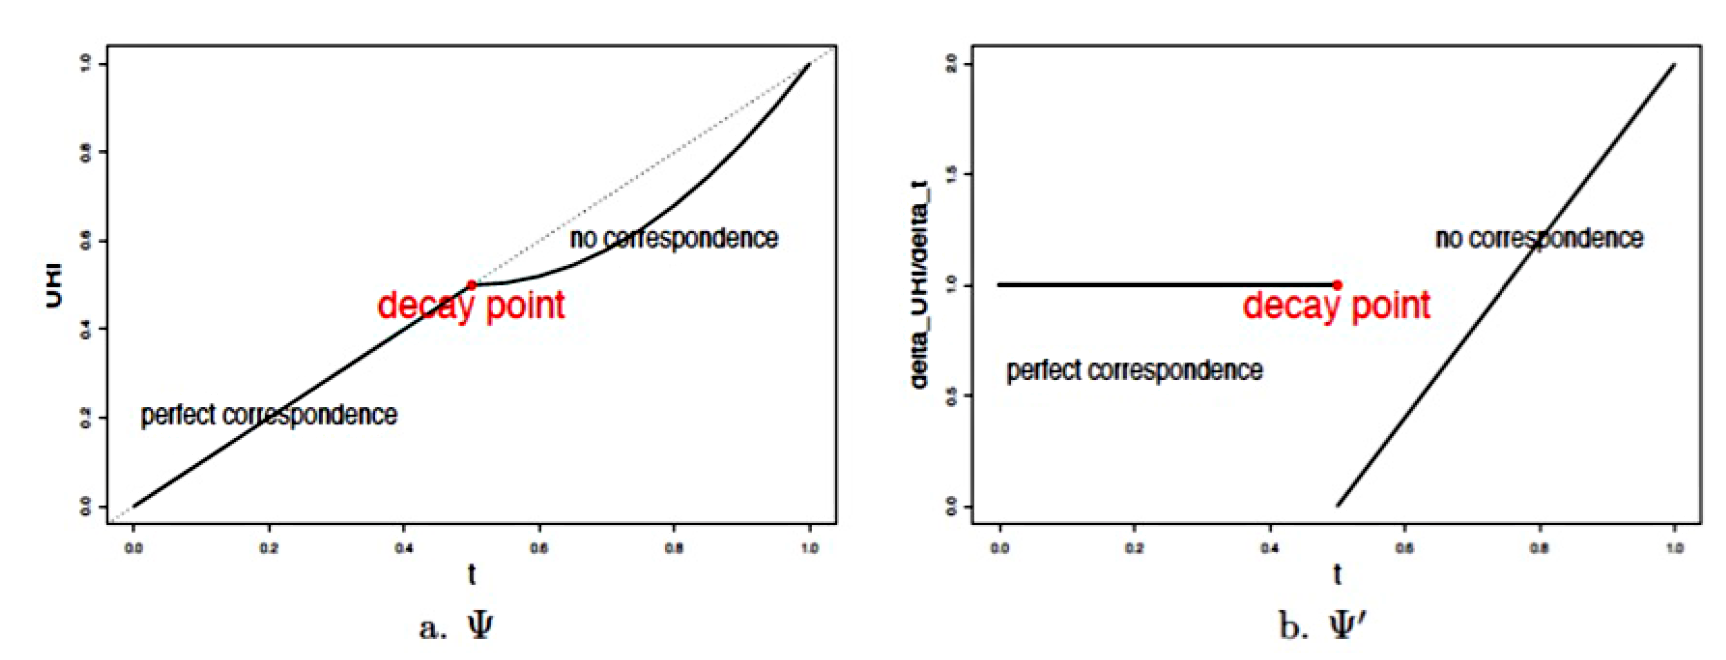
\includegraphics{images/figure1.png}
\caption{figure 1}
\end{figure}

    \textit{Figure 1: Taken from
\url{http://www.personal.psu.edu/users/q/u/qul12/IDR101.pdf}.}

    Figure 1b shows the gradient or slope of the line in Figure 1a, and so
we would expect this to be relatively flat until the decay point, when
the gradient becomes smaller.

The authors have used this principle to define numerical cutoffs on
peaks called after merging the replicates, called IDR thresholds, where
an IDR of 0.05 means that there is a 5\% chance that a peak called is
not reproducible.

    In this practical, we will again be using ChIP-Seq data for the PAX5
transcription factor, generated on the GM12878 lymphoblastoid cell line.

BAM files for the two technical replicates and a matched control Input
file have been downloaded from \url{http://www.encodeproject.org}, named
\texttt{ENCFF00NZI.bam}, \texttt{ENCFF00NZL.bam} and
\texttt{ENCFF000OCL.bam} respectively.

    We will first calculate genome-wide correlation of the read coverage of
the two PAX5 ChIP-Seq replicates, a basic measure of reproducibility
across experiments.

    \textbf{Calculate genome-wide coverages for one of the replicates,
ENCFF000NZI. The other one has already been done.}

\begin{terminalinput}
\begin{Verbatim}[commandchars=\\\{\}]
\llap{\color{black}\LARGE\faKeyboardO\hspace{1em}} genomeCoverageBed \PYZhy{}bg \PYZhy{}ibam ENCFF000NZI.bam \PYZhy{}split \PY{l+s+se}{\PYZbs{}}
        \PYZhy{}g genome/hg19.chrom.sizes \PYZgt{} ENCFF000NZI.bedgraph
\end{Verbatim}
\end{terminalinput}


    Now, we will convert the files from bedGraph
\url{https://genome.ucsc.edu/FAQ/FAQformat.html\#format1.8} genome
indexed and compressed UCSC BigWig
\url{https://genome.ucsc.edu/goldenPath/help/bigWig.html} for the same
replicate.

    \textbf{Sort ENCFF000NZI.bedgraph.}

\begin{terminalinput}
\begin{Verbatim}[commandchars=\\\{\}]
\llap{\color{black}\LARGE\faKeyboardO\hspace{1em}} \PY{n+nv}{LC\PYZus{}COLLATE}\PY{o}{=}C sort \PYZhy{}k1,1 \PYZhy{}k2,2n ENCFF000NZI.bedgraph \PYZgt{} ENCFF000NZI.sorted.bedgraph
\end{Verbatim}
\end{terminalinput}


    \textbf{Convert the bedGraph file to BigWig.}

\begin{terminalinput}
\begin{Verbatim}[commandchars=\\\{\}]
\llap{\color{black}\LARGE\faKeyboardO\hspace{1em}} bedGraphToBigWig ENCFF000NZI.sorted.bedgraph genome/hg19.chrom.sizes ENCFF000NZI.bw
\end{Verbatim}
\end{terminalinput}

\newpage

    \textbf{Finally, we compute the correlation of these two PAX5 ChIP-Seq
profiles.}

\begin{terminalinput}
\begin{Verbatim}[commandchars=\\\{\}]
\llap{\color{black}\LARGE\faKeyboardO\hspace{1em}} bigWigCorrelate ENCFF000NZI.bw ENCFF000NZL.bw
\end{Verbatim}
\end{terminalinput}


    \textbf{Q1: What is the correlation between these two samples?}

    \textbf{Q2: Is this higher or lower than you expected?}

    \textbf{Q3: What factors could explain a change in the correlation
statistic?}

    \subsection{Calculating fragment lengths from ChIP-Seq
data}\label{calculating-fragment-lengths-from-chip-seq-data}

    As part of the ChIP-seq protocol, a size selection is carried out, so
that only fragments with lengths within a specified narrow range are
selected for sequencing. This desired length is chosen by the
experimenter, and for transcription factor ChIP-seq is usually around
the size of a nucleosome (147 base pairs).

However, the true sizes chosen can differ from the targeted lengths, and
this can affect peak calling, so we try to estimate the true fragment
length using the ChIP-seq data, usually by comparing the reads aligning
to the forward and reverse strands.

As the fragments span the transcription-factor bound region, but only
the ends are sequenced, the reads map upstream of the binding site on
the forward strand and downstream on the reverse strand. One way to
calculate the fragment length is to calculate the correlation between
the read density across the two strands, when you shift one strand's
signal relative to the other by different amounts. The correlation
should have a maximum at the fragment length.

For data sets with lower enrichment, or high amplification bias, there
will also be a peak in this cross-correlation profile at a shift equal
to the read length, due to reads mapping to repeats, hence the reads on
both strands aligning to the same location.

\textbf{Phantompeakqualtools} uses the ratio of the height of the
fragment length peak and the height of the read length peak to give a
measure of sample quality.

    \begin{figure}[!h]
\centering
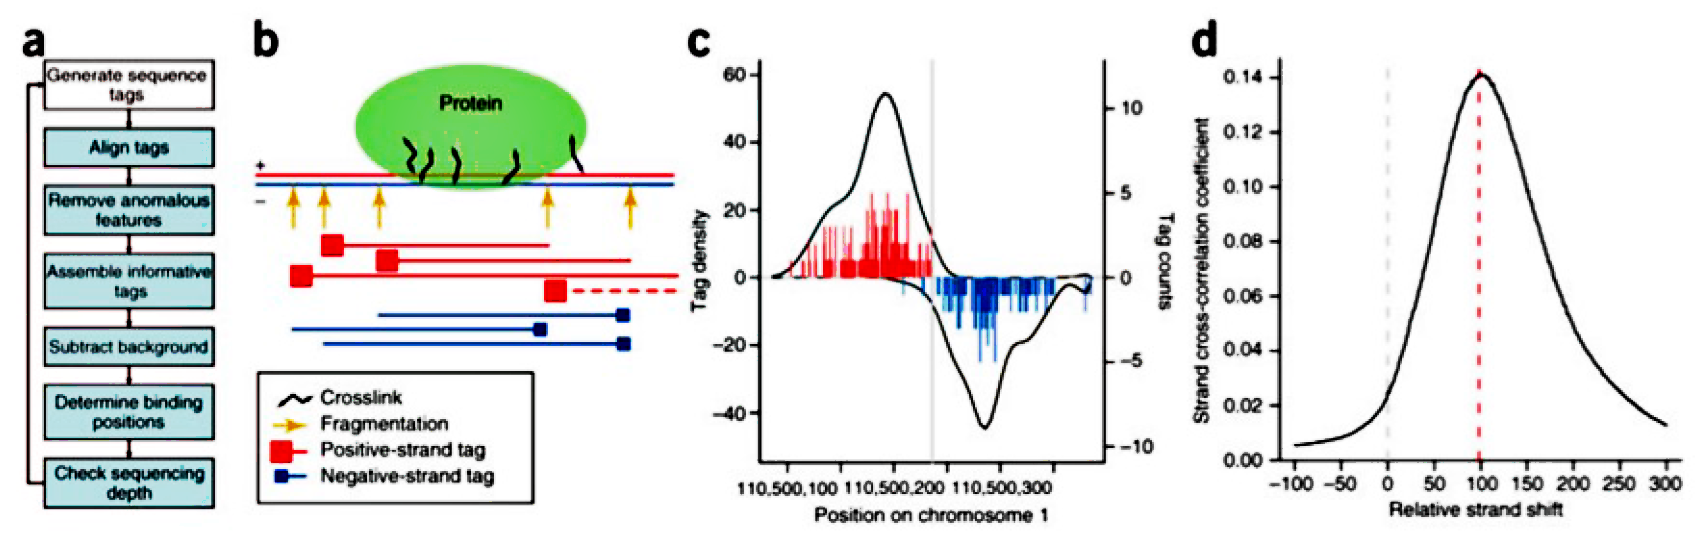
\includegraphics{images/figure2.png}
\caption{figure 2}
\end{figure}

    \textit{Figure 2: Strand-specific profile.}

\newpage

    \textbf{Calculate the fragment length for ENCFF000NZI.bam.}

\begin{terminalinput}
\begin{Verbatim}[commandchars=\\\{\}]
\llap{\color{black}\LARGE\faKeyboardO\hspace{1em}} R CMD BATCH \PYZhy{}\PYZhy{}vanilla \PYZhy{}\PYZhy{}args \PY{l+s+s1}{\PYZsq{}\PYZhy{}s=\PYZhy{}100:5:500 \PYZhy{}rf }
        \PY{l+s+s1}{    \PYZhy{}c=ENCFF000NZI.bam \PYZhy{}out=ENCFF000NZI\PYZus{}spp.out}
        \PY{l+s+s1}{    \PYZhy{}savp=ENCFF000NZI.pdf\PYZsq{}}
            /usr/local/bin/run\PYZus{}spp.R runSPP\PYZus{}ENCFF000NZI.log
\end{Verbatim}
\end{terminalinput}


    \textit{Note: We have already run run\_spp.R for the other PAX5 replicate
and the control sample.}

    Phantompeakqualtools gives a quality tag to each sample between -2 and
+2 (codes:-2:very Low, -1:Low, 0:Medium, 1:High, 2:very High).

    \textbf{Q1. What scores have our samples been given?}

    \textbf{Q2. What explanation can you think of for these scores?}

    \textbf{Q3. How could the quality of the samples be improved?}

    Now, peak calling with MACS2 is performed for both of the replicates
individually and after merging the alignments from both replicates,
using e.g. samtools merge, to create a pooled peak set.

As we have covered peak calling in the ChIP-seq practical, these data
sets are provided for you in the processed\_data/macs2 directory,
labelled ENCFF000NZI\_peaks.narrowPeak, ENCFF000NZL\_peaks.narrowPeak
and PAX5\_pooled\_peaks.narrowPeak respectively.

The narrowPeak format is an ENCODE format, using an extension of the BED
format for providing peaks and associated scores and p values. See
\url{https://genome.ucsc.edu/FAQ/FAQformat.html\#format12} for full
information.

The ChIP-seq experiment and alignment to the genome sequence is affected
by sources of artefact read mapping caused by biases in chromatin
accessibility and ambiguous alignment. These spurious regions can be
removed by filtering out any peaks that overlap a blacklist, believed to
contain experiment and cell type independent areas of high artefactual
signal. The ENCODE blacklist has been generated by combining regions of
known repeats and manually curated genomic regions of ubiquitous open
chromatin and input sequence signal. The file can be downloaded from:
\url{http://hgdownload.cse.ucsc.edu/goldenPath/hg19/encodeDCC/wgEncodeMapability/wgEncodeDacMapabilityConsensusExcludable.bed.gz}

    \textbf{We now remove any peaks which overlap with the ENCODE
blacklist.}

\begin{terminalinput}
\begin{Verbatim}[commandchars=\\\{\}]
\llap{\color{black}\LARGE\faKeyboardO\hspace{1em}} bedtools intersect \PYZhy{}a ENCFF000NZI\PYZus{}peaks.narrowPeak \PY{l+s+se}{\PYZbs{}}
        \PYZhy{}b wgEncodeDacMapabilityConsensusExcludable.bed \PY{l+s+se}{\PYZbs{}}
        \PYZhy{}v \PYZgt{} ENCFF000NZI\PYZus{}peaks\PYZus{}filtered.narrowPeak
\end{Verbatim}
\end{terminalinput}


    Next, we need to sort the peak files into significance order. For MACS2,
the p-value works best as the ranking for the IDR procedure. See
\url{https://sites.google.com/site/anshulkundaje/projects/idr\#TOC-Peak-callers-tested-with-IDR}
for the best measures to use with other peak callers.

\newpage

    \textbf{Here, we sort by p value and then use the 100,000 most
significant peaks.}

\begin{terminalinput}
\begin{Verbatim}[commandchars=\\\{\}]
\llap{\color{black}\LARGE\faKeyboardO\hspace{1em}} sort \PYZhy{}k 8nr,8nr ENCFF000NZI\PYZus{}peaks\PYZus{}filtered.narrowPeak \PY{p}{|} \PY{l+s+se}{\PYZbs{}}
        head \PYZhy{}n \PY{l+m}{1000} \PYZgt{} ENCFF000NZI\PYZus{}top100000\PYZus{}peaks.narrowPeak
\end{Verbatim}
\end{terminalinput}


\begin{terminalinput}
\begin{Verbatim}[commandchars=\\\{\}]
\llap{\color{black}\LARGE\faKeyboardO\hspace{1em}} sort \PYZhy{}k 8nr,8nr ENCFF000NZL\PYZus{}peaks\PYZus{}filtered.narrowPeak \PY{p}{|} \PY{l+s+se}{\PYZbs{}}
        head \PYZhy{}n \PY{l+m}{100000} \PYZgt{} ENCFF000NZL\PYZus{}top100000\PYZus{}peaks.narrowPeak
\end{Verbatim}
\end{terminalinput}


\begin{terminalinput}
\begin{Verbatim}[commandchars=\\\{\}]
\llap{\color{black}\LARGE\faKeyboardO\hspace{1em}} sort \PYZhy{}k 8nr,8nr PAX5\PYZus{}pooled\PYZus{}peaks\PYZus{}filtered.narrowPeak \PY{p}{|} \PY{l+s+se}{\PYZbs{}}
        head \PYZhy{}n \PY{l+m}{100000} \PYZgt{} PAX5\PYZus{}pooled\PYZus{}top100000\PYZus{}peaks.narrowPeak
\end{Verbatim}
\end{terminalinput}


    \textbf{Finally, we can perform the IDR analysis on the peaks called in
the two technical replicates.}

\begin{terminalinput}
\begin{Verbatim}[commandchars=\\\{\}]
\llap{\color{black}\LARGE\faKeyboardO\hspace{1em}} Rscript batch\PYZhy{}consistency\PYZhy{}analysis.r \PY{l+s+se}{\PYZbs{}}
        ENCFF000NZI\PYZus{}top100000\PYZus{}peaks.narrowPeak \PY{l+s+se}{\PYZbs{}}
        ENCFF000NZL\PYZus{}top100000\PYZus{}peaks.narrowPeak \PY{l+s+se}{\PYZbs{}}
        \PYZhy{}1 ENCFF000NZI\PYZus{}vs\PYZus{}ENCFF000NZL \PY{l+m}{0} F p.value
\end{Verbatim}
\end{terminalinput}


    \textbf{Now, produce a graphical representation of the IDR output.}

\begin{terminalinput}
\begin{Verbatim}[commandchars=\\\{\}]
\llap{\color{black}\LARGE\faKeyboardO\hspace{1em}} Rscript batch\PYZhy{}consistency\PYZhy{}plot.r \PY{l+m}{1} PAX5\PYZus{}2Reps ENCFF000NZI\PYZus{}vs\PYZus{}ENCFF000NZL
\end{Verbatim}
\end{terminalinput}


    \textbf{As the output of the above command (idr/PAX5\_2Reps-plot.ps)
cannot be opened on these PCs, convert it to a PDF file.}

\begin{terminalinput}
\begin{Verbatim}[commandchars=\\\{\}]
\llap{\color{black}\LARGE\faKeyboardO\hspace{1em}} ps2pdf idr/PAX5\PYZus{}2Reps\PYZhy{}plot.ps idr/PAX5\PYZus{}2Reps\PYZhy{}plot.pdf
\end{Verbatim}
\end{terminalinput}


    \subsection{Understanding the IDR output
plot}\label{understanding-the-idr-output-plot}

The top left of the five plots is the equivalent of Figure 1a,
considering all peaks, and the top centre figure is the equivalent of
Figure 1a, only considering overlapping peaks called in both replicates.
The number of peaks in common in the top X peaks of both replicates is
shown in each case.

The two figures below these plot the slope (gradient) of the above
graph, again for all peaks and matched peaks respectively. The top right
figure shows the IDR value increasing as the rank of the peaks goes
down. You can use this plot to see how many peaks pass the IDR test for
different threshold values. A good value for the IDR cutoff in this case
is 0.05. See also
\url{http://www.personal.psu.edu/users/q/u/qul12/IDR101.pdf}.

    \textbf{Q4. How reproducible are the peaks called in these two technical
replicates for PAX5 binding in the GM12878 cell line?}

    \textbf{Q5. What factors could lower the reproducibility between two
ChIP-seq experiments?}

\newpage

    \textbf{Open the file ENCFF000NZI\_vs\_ENCFF000NZL-overlapped-peaks.txt
to see how many peaks pass the IDR threshold of 0.05.}

\begin{terminalinput}
\begin{Verbatim}[commandchars=\\\{\}]
\llap{\color{black}\LARGE\faKeyboardO\hspace{1em}} less ENCFF000NZI\PYZus{}vs\PYZus{}ENCFF000NZL\PYZhy{}overlapped\PYZhy{}peaks.txt
\end{Verbatim}
\end{terminalinput}


    We now use this number of reproducible peaks, generated on the
individual replicate peak calls, to select the same number of peaks from
the pooled replicates peak calls.

    \textbf{Replace {[}numPeaks{]} with the number of peaks passing the 0.05
threshold in the following command.}

    head -n {[}numPeaks{]} PAX5\_pooled\_top100000\_peaks.narrowPeak
\textgreater{} PAX5\_pooled\_macs2.conservative.narrowPeak

    This file is the final output of IDR, generating a final peak set on the
merged replicates. IDR can also be used with more than two replicates.
In this case, the IDR procedure is followed for all pairwise
comparisons, and the highest number of peaks passing the IDR cutoff is
used for filtering the pooled peak list.

    CONGRATULATIONS! You've made it to the end of the practical. We hope you
enjoyed it!

    \subsection{Bonus Exercise I}\label{bonus-exercise-i}

The IDR statistics can also be used to flag data sets with low
reproducibility. This may be due to one of the two replicates being of
lower ChIP enrichment, hence having a high signal-noise ratio. In this
case, the standard IDR protocol would record few reproducible peaks,
despite one replicate having high information content.

ENCODE has developed a rescue strategy in this case by using
pseudo-replicates. These pseudo-replicates are generated by pooling all
the reads, and then randomly splitting them into two files. These
pseudo-replicates do not represent true biological or experimental
replicates, but attempt to model the stochastic noise in the sampling of
sequenced reads from a population of fragments.

The pseudo-replicates analysis uses a lower IDR threshold than
biological replicates, due to the reduced noise, typically 0.0025.

\textbf{Using
\url{https://sites.google.com/site/anshulkundaje/projects/idr} and
modifiying the code above, run the IDR analysis for pseudo-replicates of
the GM12878 PAX5 ChIP-seq data.}

\textbf{Q6: Does the IDR method select more peaks using the original
technical replicates or the pseudo-replicates?}


    % Add a bibliography block to the postdoc



\end{document}
